%% Optimask Commands and Scripts
%% Created: 2017-05-15; Updated: 2017-07-15;
%% by Henghua DENG, hdeng@optixera.com

\resetdatestamp %Date Stamp--Only use when custom package datestamp.sty is used.

%\part{Optimask Layout Design} \label{PartMaskDesign}
%本部分介绍Optimask版图设计软件基本框架,具体功能实现,主要界面,命令行及编程输入等等。

\chapter{Optimask Commands and Scripts} \label{ChMaskCmdScript}
%======================================================================
%Heading Settings:
\markboth{Chapter~\thechapter.~Command~Script}{} %\leftmark calls #1 parameter
%\markright{ } % new right header. Only used for two-side documents.

\pagestyle{fancy}
\fancyhead[RO,RE]{}
\fancyhead[LE]{\MakeUppercase{\leftmark}}
\fancyhead[LO]{\MakeUppercase{\rightmark}}
\fancyfoot[C]{\thepage}
%%\fancyfoot[L]{\today}

命令(Command)和脚本(Script)是非常有用的功能。目前其他软件的命令和脚本功能,或者功能太弱,或者太复杂,或者太难使用。在Optimask软件下,我们将定义非常简单高效的命令和脚本。

%======================================================================
\section{命令和脚本的基本原则} \label{SectCmdRule}
%======================================================================
Optimask软件中,命令和脚本的基本原则是简单高效易使用,对于用户而言是非常浅显易记的语言(Plain Language)。命令、脚本或宏的输入是在CodeDock命令输入窗口(见Figure (\ref{FigCodeDock}))交互输入和执行的。

\begin{figure}[htb!p] %h--here, t--top, b--bottom, p--page;
	\centering
	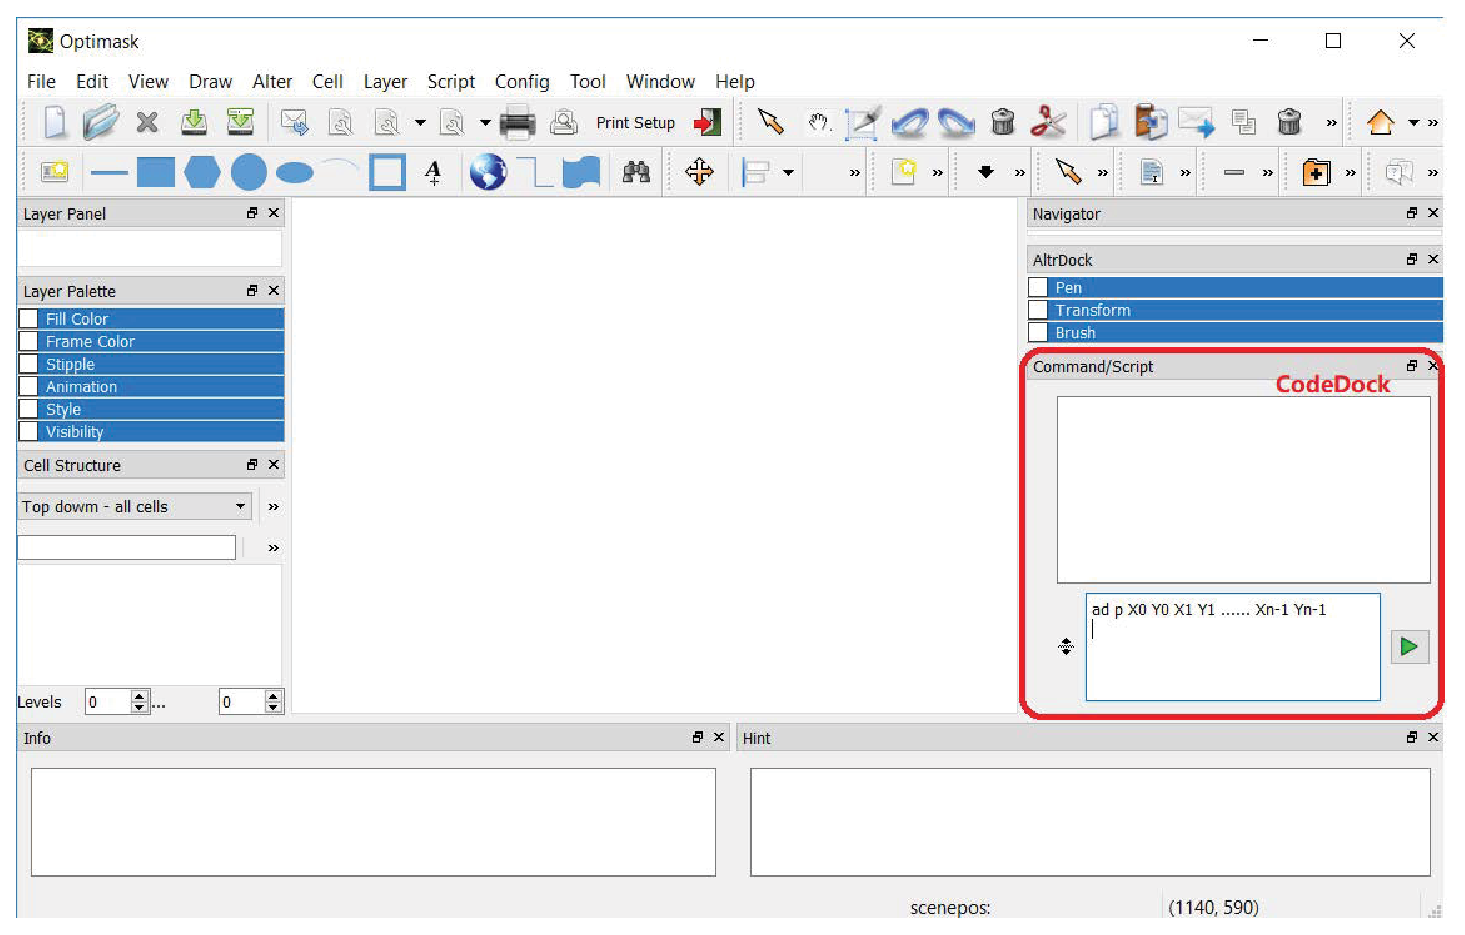
\includegraphics[width=4in]{./Layout/FigsCmd/CodeDock.eps}
	\caption{CodeDock for Command/Script/Macro input.}
	\label{FigCodeDock}
\end{figure}

\subsection{实时输入和文件运行} \label{SectCmdInput} 
允许实时输入,允许多行命令同时输入和执行,允许存储命令记录为文档,允许导入命令脚本文件直接执行。

文件存储为文本文件,便于用户阅读和修改。

命令可以通过命令输入窗口交互输入执行,也可以通过导入命令文件后执行。界面窗口有历史命令导出为文件的按钮,也有导入命令文件的按钮。导入命令文件之后可以点击执行(RUN)按钮。

此外还有一个选择是可以通过在命令输入窗口输入@符号加上文件名(可以不指定文件后缀),即文件运行使用\emph{@文件名})。比如如果命令文件名为AWG.cmd,那么在命令输入栏输入
\begin{verbatim} @AWG \end{verbatim} 
就等同于打开(OPEN)此文件后再执行(RUN)。

注意,命令文件的文本里面同样可以允许\emph{@文件名}的使用,即允许文件的嵌套调用。这样就大大扩展了命令和脚本文件的使用灵活性和功能性。

\subsection{命令注释} \label{SectCmdComment} 
文件中,注释允许多重注释符号,以扩展代码的灵活性和兼容性。允许的注释符号包括:
%%标准C/C++注释符(//, /* */)亦即Java注释符(//, /* */), Matlab注释符(\%)亦即\LaTeX注释符(\%), Python注释符(\#), DOS注释符(!)。
\begin{itemize}
	\item 标准C/C++注释符(//, /* */),亦即Java注释符,及L-Edit的T-Cell注释符
	\item Matlab注释符(\%),亦即LaTeX注释符(\%)
	\item Python注释符(\#)
	\item DOS注释符(!),亦即IC Editor注释符(!)
\end{itemize}

这些注释符号可以随意出现的命令和文件的任何位置。所有这些注释符号以及直到行末的文本在编译时都将被忽略。

\subsection{命令解析} \label{SectCmdIntrp} 
命令解析主要在后台自动进行。好的解析可以允许用户有适当的自由度,在适当的时候允许用户调整命令格式,以简化用户的计算和简化输入。
\subsubsection{模糊识别和自动输入} \label{SectCmdFuzy} 
命令和脚本解析允许模糊识别功能,且不分大小写。
比如添加多边形,
Add Polygon at (X0, Y0),  (X1, Y1), ......, (Xn-1, Yn-1);
等同于
ad p X0 Y0 X1 Y1 ...... Xn-1 Yn-1
如果以p开头的命令只有polygon。
假设以p开头的命令只有polygon和polyline,那么必须用户输入到polyg才可以区别。以此类推。
不区别大小写。
对于坐标组,是否有括符 (), [], \{\}都没关系,是否有逗号或分号分隔都没关系。

已添加矩形为例,命令如下:
Add Rectangle
Add Rect
Add Box
坐标只需要
X0 Y0 X1 Y1 
即左下角和右上角的两个定点坐标。
如果add已经可以用ad足够区分,如果没有R或B开头的关键词跟在Add 后面,那么
ad b
也可以工作。

\subsubsection{基本格式和变形格式} \label{SectCmdForms} 
对于每个命令,缺省有一个基本格式,同时可能有存在的变形格式。

对于任何一个基本图形,需要确定一个基本格式,比如
add box X0 Y0 X1 Y1 (W)
为添加矩形的基本命令格式。它确定一个(X0,Y0),(X0,Y1),(X1,Y1),(X0,Y1)的矩形,其各边均与(X,Y)坐标平行。

此基本格式不需要输入额外的变量名字,即后面的参数全为数字即可自动解析。但是如果希望以其他变形格式输入时,就需要输入变量名字和数值。比如

add box X0 Y0 X1 Y1 (W) rotateangle=90deg (rotatecenter=(Ox,Oy))

就会将此box对应rotatecenter旋转rotateangle。
其中rotatecenter缺省为box的中心点,如果用户指定rotatecenter=(Ox,Oy)那么就沿此(Ox,Oy)进行旋转。

同一个命令可以有多个变形格式,比如

add box Origin=(Ox,Oy) Width=10 Height=20 (W)

就会建立一个以(Ox,Oy)为中心,长度为10,高度为20的矩形,线宽W缺省为0。
或者

add box Base=(X,Y) Width=10 Height=20 (W)

就会建立一个以(X,Y)为左下角,长度为10,高度为20的矩形,线宽W缺省为0。

变形格式可以在后台全部自动转换为基本格式进行处理。如果是图形窗口(GUI)读取的命令,基本上可以转换为基本格式自动存储和计算。

\subsubsection{复合格式} \label{SectCmdCmb} 
同时可以允许有复合格式,即两个命令的混合。

比如命令1:
add box X0 Y0 X1 Y1 (W) 为添加矩形,

而命令2:
rotate angle center
将图形对应旋转中心center 坐标(Ox,Oy),旋转angle角度的操作。
那么
add box X0 Y0 X1 Y1 (W) rotate angle center
即为将此矩形产生和同时进行旋转操作。

其实该复合格式等同于同时执行两条命令:

add box X0 Y0 X1 Y1 (W)

rotate angle center

操作的目标缺省定义为最近绘制的那个图形。

\subsection{参数惯例} \label{SectCmdConvention} 
建议写程序代码时参数命名始终遵循下面这些惯例。但是对于用户是透明的。
\begin{enumerate}
	\item 大写(X,Y)为绝对坐标值,小写(x,y)为相对坐标值。换算关系为(X,Y)=(Ox,Oy)+(x,y),其中(Ox,Oy)为相对坐标系的原点在绝对坐标系中的坐标位置。
	\item angle为角度(degree),ang为弧度(radian)。二者换算关系为$ang=\dfrac{angle*\pi}{180}$和$angle=\dfrac{ang*180}{\pi}$。如果定义$deg=\dfrac{\pi}{180}$和$rad=\dfrac{180}{\pi}$,那么简单地通过2*deg就将角度$2^{\circ}$转换成弧度$\dfrac{\pi}{90}$,而$\dfrac{\pi}{4}*rad$就将弧度$\dfrac{\pi}{4}$转换成角度$45^{\circ}$。
	\item res为角弧精度(即对于弧线,变为多边形时,隔几度一个点),缺省单位为弧度(radian),缺省值为2*deg。
	\item (Ox,Oy)一般表示坐标系原点或圆心的绝对坐标位置。
	\item R为Radius(半径),等于直径的一半。
	\item W为线宽,缺省为0,表示没有线宽。(比如Add Circle如果W=0,那么产生实心圆形;否则就产生有线宽的圆环,内径的半径为R-0.5W,外径的半径为R+0.5W。)
\end{enumerate}

%======================================================================
\section{命令总览} \label{SectCmdCtgr} %Command Category
%======================================================================
命令总览可参考思维导图(XMind)文件
\begin{verbatim} \optixera\Docs\Optimask_File_Format.xmind \end{verbatim}。
命令总览见Figure (\ref{FigCmdOverview})所示,包含几个基本类别,如编辑、绘制、构元、视图、特性、变化等。下面依次介绍各类命令下的基本命令。
\begin{figure}[htb!p] %h--here, t--top, b--bottom, p--page;
	\centering
	\subfigure[Command Category(命令类别)] {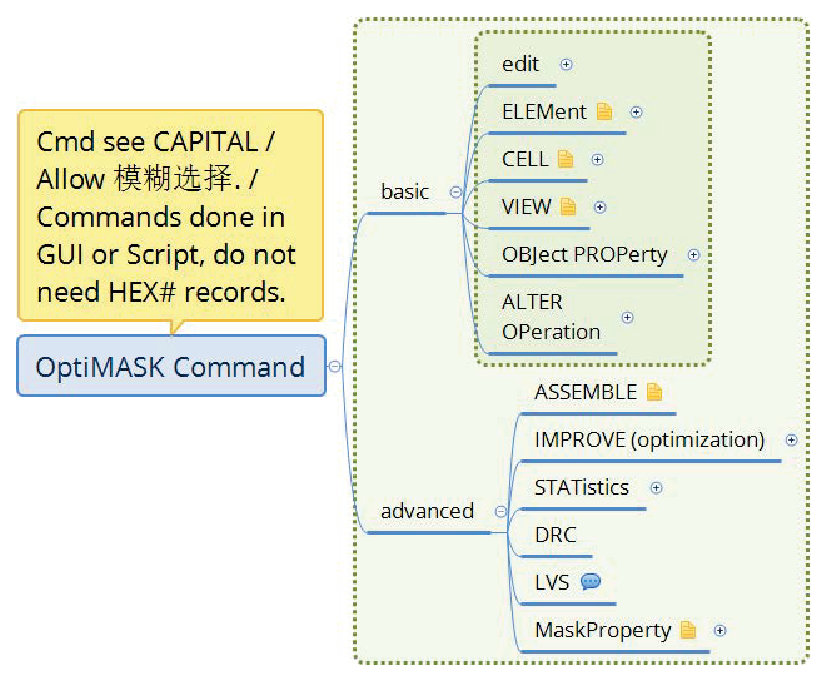
\includegraphics[width=3in]{./Layout/FigsCmd/CmdCategory.eps}
		\label{FigCmdCtgry}}
	\hfill
	\subfigure[Command Minimum Set(命令最小子集)] {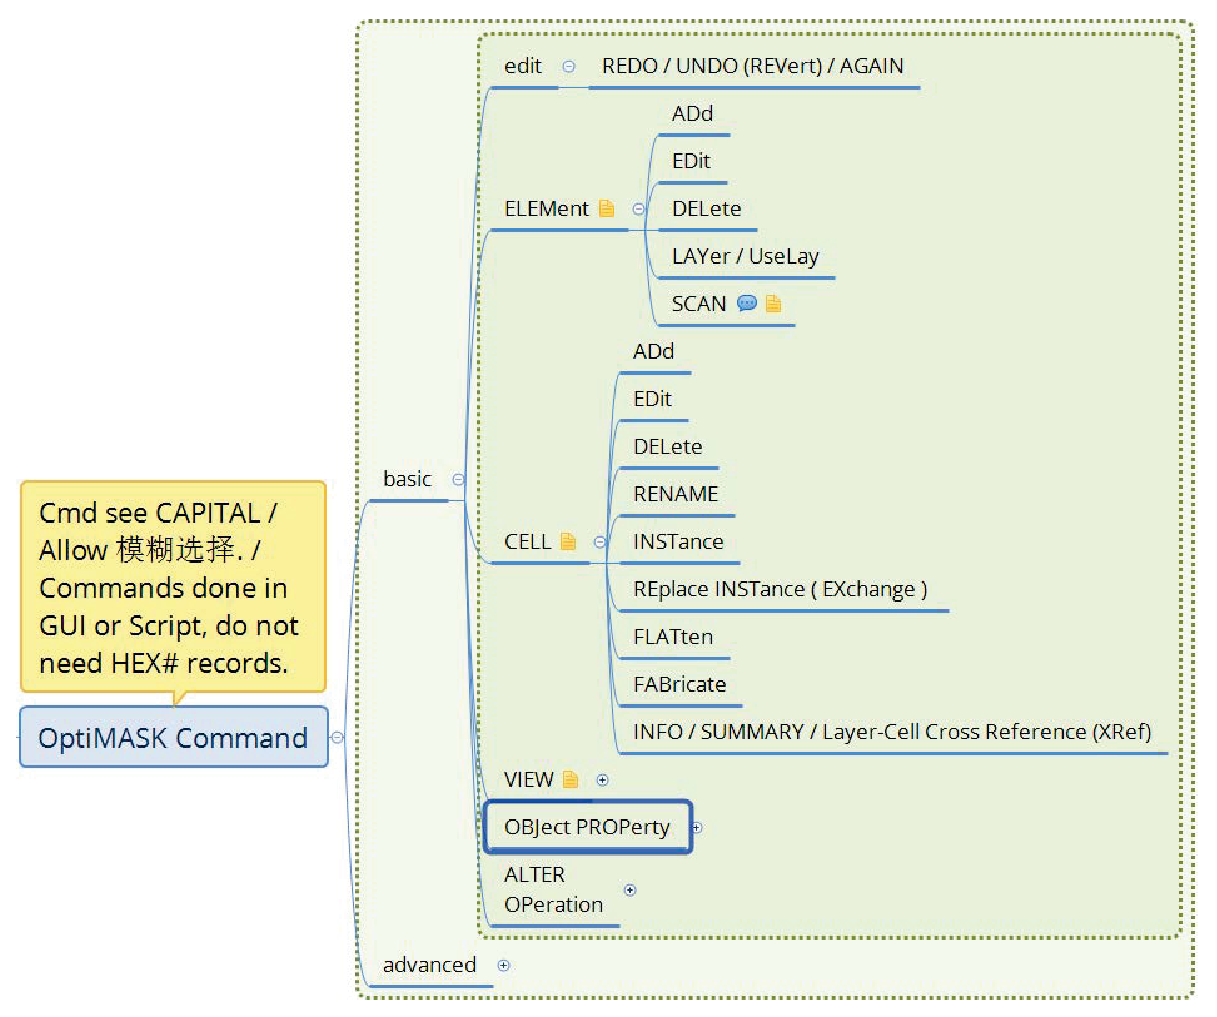
\includegraphics[width=3in]{./Layout/FigsCmd/CmdMinSet.eps}
		\label{FigCmdMinSet}}
	\caption{Overview of Commands 命令总览。}
	\label{FigCmdOverview}
\end{figure}

\subsection{编辑(Edit)} \label{SectCmdEdit}
操作REDO(AGAIN) / UNDO (REVert),主要针对最后一个命令行。这些对应界面的撤销和重复的动作。

Edit(编辑)的具体操作可以针对某个基本图元(Element),也可以针对某个复合构元(Cell),相应的Edit(编辑)将在对应的命令类别下面单独详细阐述。

\subsection{基本图形(Element)} \label{SectCmdDraw}
绘制基本图形(Draw Element)的操作命令见Figure \ref{FigCmdElem}。
\begin{figure}[htb!p] %h--here, t--top, b--bottom, p--page;
	\centering
	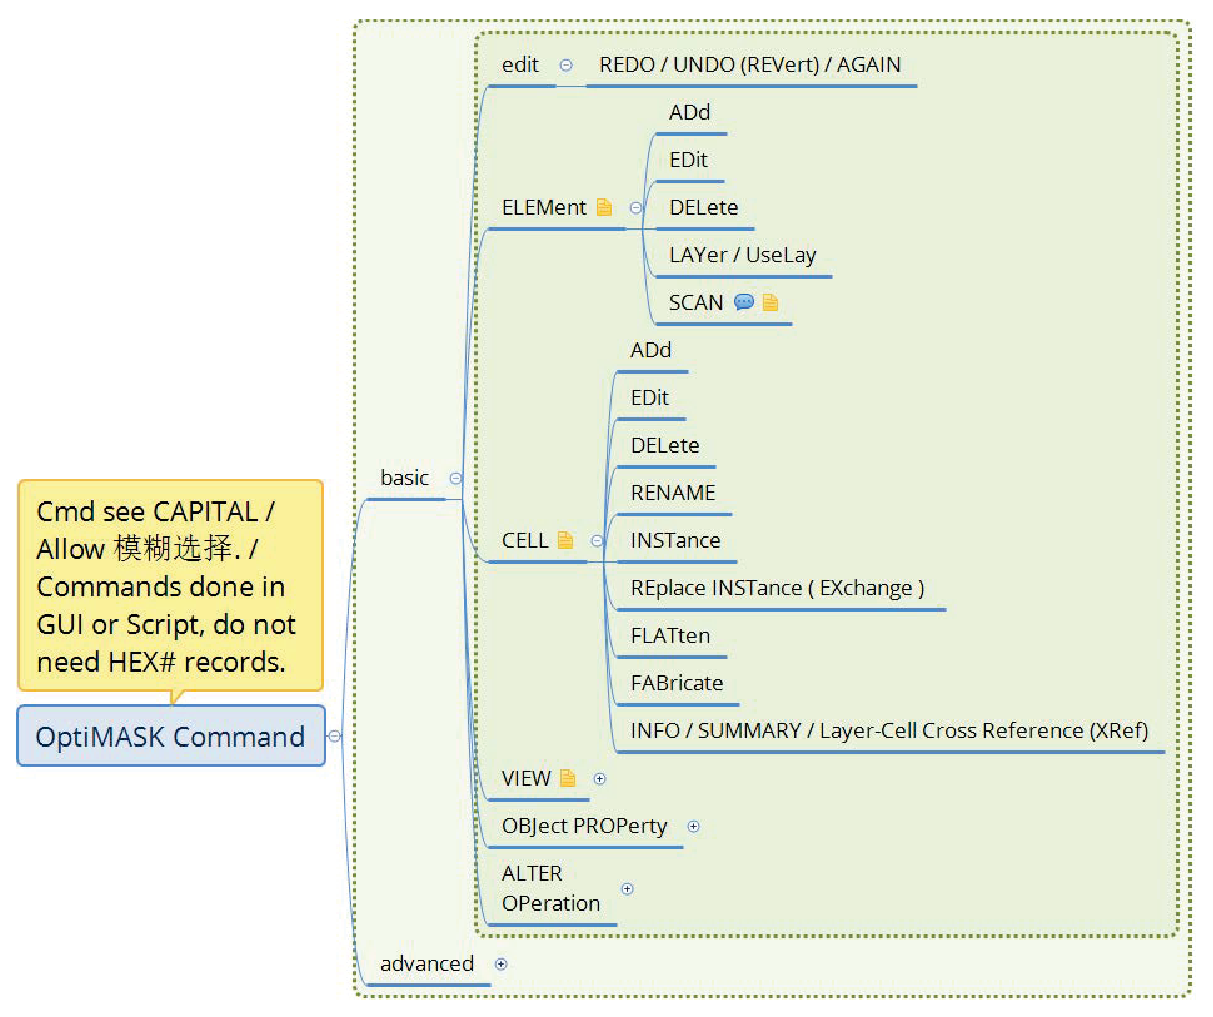
\includegraphics[width=4in]{./Layout/FigsCmd/CmdBasicElement.eps}
	\caption{Commands to Create Basic Elements 绘制基本图形命令。}
	\label{FigCmdElem}
\end{figure}
可以有Add(添加)(Draw),Edit(编辑),Delete(删除),Layer(构层)(即UseLayer,使用层号),以及高级功能Scan(扫描)。

\subsubsection{添加图元(Add)} \label{SectCmdAdd}
添加图元(Add/Draw Element)可以使用Add(添加)命令。添加的常用基本图形的基本格式示例如下
\begin{itemize}
	\item add box X0 Y0 X1 Y1 (W)
	\item add polygon X0 Y0 X1 Y1 ...... Xn-1 Yn-1 (W)
	\item add circle Ox Oy R (res) (W)
	\item add arc Ox Oy R ang1 ang2 (res) (W) 
	\item add Figure (\ref{FigExtRefElem})下的更复杂图元。
\end{itemize}
其中括弧框中的变量(比如(W))为可选项;若不存在则使用缺省值(比如(W=0))。非括弧框中的变量为必须提供的变量参数。

\begin{figure}[htb!p] %h--here, t--top, b--bottom, p--page;
	\centering
	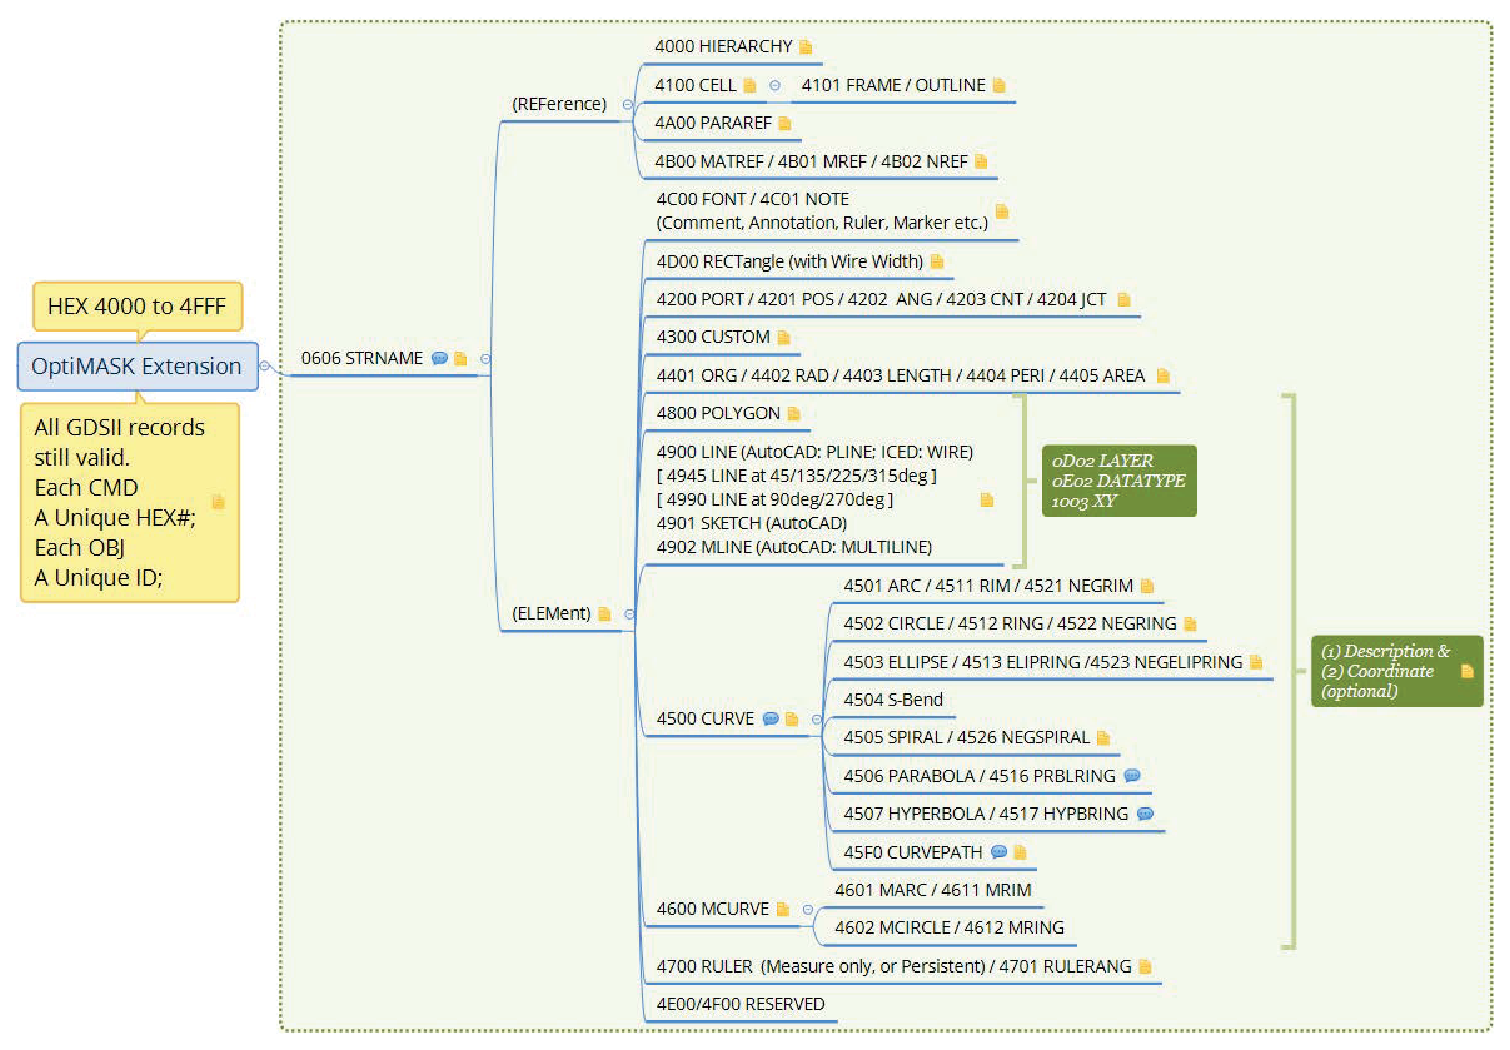
\includegraphics[width=4in]{./Layout/FigsCmd/Optimask_Ext_REF_ELEM.eps}
	\caption{Optimask Extension (相对于GDSII的扩展)。}
	\label{FigExtRefElem}
\end{figure}

比如,添加圆形图形命令

ad circle Ox Oy R (res) (W)

其中 (Ox, Oy) 为圆心,R为半径,res为精度。
当W不为0时,相当于

ad ring Ox Oy R res W

其中(Ox, Oy) 为圆心,R为半径,W为宽度,res为精度。

\subsubsection{编辑图元(Edit)} \label{SectCmdEditElem}
编辑图元(Edit Element)可以使用Edit(编辑)命令。Edit的目标不限于图元(Element),也可以是构元(Cell)。

因为图元(Element)通常太多,且没有命名,所以无法通过名字来编辑图元。因此,可以通过图元的标号来编辑,或者通过选择来编辑,比如:

\begin{itemize}
	\item edit ID=(12456, 25, 36) (编辑指定ID的图元们,允许多选,但不推荐)
	\item edit select (编辑已经选中的图元们;若没有选中任何图元或构元,则进入选择模式后编辑)
	\item edit select in  (然后等待用户通过鼠标框选后编辑)
	\item edit cell CELLNAME (编辑指定名字的构元,暂不允许多选)
	\item edit cell CELLID (编辑指定ID的构元,暂不允许多选)
\end{itemize}
注意,最后一个命令为编辑构元,详细请参见分节\ref{SectCmdEditCell}。

\subsubsection{删除图元(Delete)} \label{SectCmdDelElem}
删除选中的图元。
\begin{itemize}
	\item delete select (删除当前激活的构元上选中的图形)
	\item delete all (删除当前激活的构元上所有的图形)
	\item delete layer LAYERID (or LAYERNAME) (删除当前激活的构元上的指定层上的图形)
	\item delete cell CELLID (or CELLNAME) (删除指定的构元;同时从目录树上删除;清除内存和存储。)
\end{itemize}

\subsubsection{选择图元(Select)} \label{SectCmdSelElem}
选中和取消选中的操作命令:
\begin{itemize}
	\item select in    (面积选中)
	\item select near  (边框选中)
	\item select all   (全部选中)
	\item deselect in
	\item deselect near
	\item deselect all
\end{itemize}

选择必定是通过一个Box(Frame)来实现的,或者通过鼠标的两次点击(两个不同的点可以确定一个无旋转的矩形区域,即与X,Y坐标平行),或者通过命令行指定这个矩形区域。

1. 边框选中 对应 Select Near:即只要这个选择框碰到的图元和构元,就被选中。或者说,只要图元或构元的边框(Frame),和这个指定的选择框有交集,那么就被选中。

2. 面积选中 对应 Select In 或者 Select Box ,只有完全落在选择框限定的区域内的图元和构元,才被选中。或者说,必须图元或构元的边框(Frame)完全落在选择框内,才被选中。

\subsection{构层(Layer)} \label{SectCmdLayer}
构层(Layer)命令缺省将绘制设定在指定的构层上

Layer LAYERID (等同于 Use Layer LAYERID)

或者

layer LAYERNAME (等同于 Use Layer LAYERNAME)

比如layer 10, 那么,后面所有的图形将是绘制在GDSII第10层上。或者layer METAL,那么所有的图形将是绘制在构层METAL上。

同时可以允许基本的构层(Layer)操作,比如

layer map SOURCE to DESTINATION (将所有选中的在源构层上的图形对应转换到目标构层上。该操作是一一对应的。)

layer combine (LayerList) to DESTINATION (将所有选中的在源构层清单上的图形对应转换到目标构层上。该操作是合并多层到一层的。)

layer (LayerList) select all (Layer和Select命令的复合格式;限于当前构元。)

select layer (LayerList) all (Layer和Select命令的复合格式;限于当前构元。)

layer (LayerList) deselect all (Layer和DeSelect命令的复合格式;限于当前构元。)

deselect layer (LayerList) all (Layer和DeSelect命令的复合格式;限于当前构元。)

layer (LayerList) delete all (Layer和Delete命令的复合格式;限所有选中的构元。)

delete layer (LayerList) all (Layer和Delete命令的复合格式;限所有选中的构元。)

\subsection{构元(Cell)} \label{SectCmdCell}

\subsubsection{新建构元(Add Cell)} \label{SectCmdNewCell}
新建构元(Add Cell 或者 New Cell)。新建指定名字的构元,CellID由程序自动给出。
\begin{itemize}
	\item cell CELLNAME 
	\item (add) cell CELLNAME
	\item (new) cell CELLNAME
\end{itemize}

\subsubsection{编辑构元(Edit Cell)} \label{SectCmdEditCell}
如分节\ref{SectCmdEditElem}所列,Edit的目标不限于图元(Element),也可以是构元(Cell)。
\begin{itemize}
	\item edit cell CELLNAME (编辑指定名字的构元,暂不允许多选)
	\item edit cell CELLID (编辑指定ID的构元,暂不允许多选)
\end{itemize}
进入编辑状态后,用户进行修改后,可以按保存(Save,Ctrl+S)后退出,或者放弃修改而退出(Quit,Ctrl+Q)(即不保存)。在退出(Quit,Ctrl+Q)命令执行时会弹出确认对话框,是否确定放弃修改?如果想强制退出,不保存修改,也不弹出对话确认框,那么可以使用离开(Leave)命令。

\subsubsection{复制构元(Copy Cell)} \label{SectCmdCopyCell}
复制构元(Duplicate Cell 或者 Copy Cell)。复制指定名字的构元,NEWCellNAME若不存在就由程序自动给出。CellID由程序自动给出。
\begin{itemize}
	\item duplicate cell CELLNAME (to) NEWCELLNAME 
	\item copy cell CELLNAME (to) NEWCELLNAME
	\item clone cell CELLNAME (to) NEWCELLNAME
\end{itemize}

\subsubsection{重命名构元(Rename Cell)} \label{SectCmdRenameCell}
重命名构元(Rename Cell)。重新命名指定名字的构元,CellID不变。NEWCellNAME若已经存在就程序对话框提示,然后不进行重命名。
\begin{itemize}
	\item rename cell CELLNAME (to) NEWCELLNAME 
\end{itemize}

\subsubsection{引用构元(Instance Cell)} \label{SectCmdCallCell}
引用构元(Instance Cell)。在当前母构元中,引用的子构元CELLNAME。
\begin{itemize}
	\item instance cell CELLNAME (to) (ParentCELLNAME) 
\end{itemize}

\subsubsection{交换构元(Exchange Cell)} \label{SectCmdExchCell}
交换构元(Exchange Cell)。交换两个构元的名字,各自CellID和内容都不改变。这样对于Intance失误后修改非常方便。
\begin{itemize}
	\item exchange cell CELLNAME1 CELLNAME2
\end{itemize}

\subsubsection{替换构元(Replace Cell)} \label{SectCmdReplCell}
替换构元(Replace Cell)。 在当前母构元中,替换引用的子构元的名字,将原先引用的子构元CELLNAME1替换成子构元CELLNAME2。两个子构元CELLNAME1和CELLNAME2的各自CellID和内容都不改变,但是当前母构元内容修改了。这样对于Intance失误后修改非常方便。
\begin{itemize}
	\item Replace cell CELLNAME1 CELLNAME2 (in) (ParentCELLNAME) 
\end{itemize}

\subsubsection{弄平构元(Flatten Cell)} \label{SectCmdFlatCell}
平整(Flat)就是指该构元没有层次结构,全部由基本图形构成,没有引用任何其他构元。
将有层次结构的构元变成平整(Flat)的构元这个动作被称为弄平(Flatten)。

弄平构元(Flatten Cell)将当前母构元中所有子构元(包括子子构元)的图形全部弄平整,使之只存在基本图形,而不再有子构元以及从属结构(Hirearchy Structure)关系。母构元存储空间可能需要增大,对之前所调用的子构元的再次修改将不再影响此平整(Flat)的母构元。
\begin{itemize}
	\item Flatten cell CELLNAME 
	\item Flatten cell CELLIDLIST 
\end{itemize}

\subsubsection{制造构元(Fabricate Cell)} \label{SectCmdFabCell}
制造构元(Fabricate Cell)即将所有自定义的图形转换成GDSII的多边形格式存储。
\begin{itemize}
	\item Fabricate cell CELLNAME
\end{itemize}

\subsubsection{构元信息(Info Cell)} \label{SectCmdInfoCell}
构元信息(Info Cell)显示INFO / SUMMARY / Layer-Cell Cross Reference (XRef)。多少构层,多少子构元,多少级引用,多少多边形,占用多少面积,绕线周长,等等。

\begin{itemize}
	\item Info cell CELLNAME
\end{itemize}

\subsection{视图(View)} \label{SectCmdView}
视图(View)的基本操作命令见Figure \ref{FigCmdView}。因为主要是屏幕视图的操作,大部分命令使用鼠标、菜单、或快捷键操作即可。简单常用的视图操作还是需要可以用命令行执行的。
\begin{figure}[htb!p] %h--here, t--top, b--bottom, p--page;
	\centering
	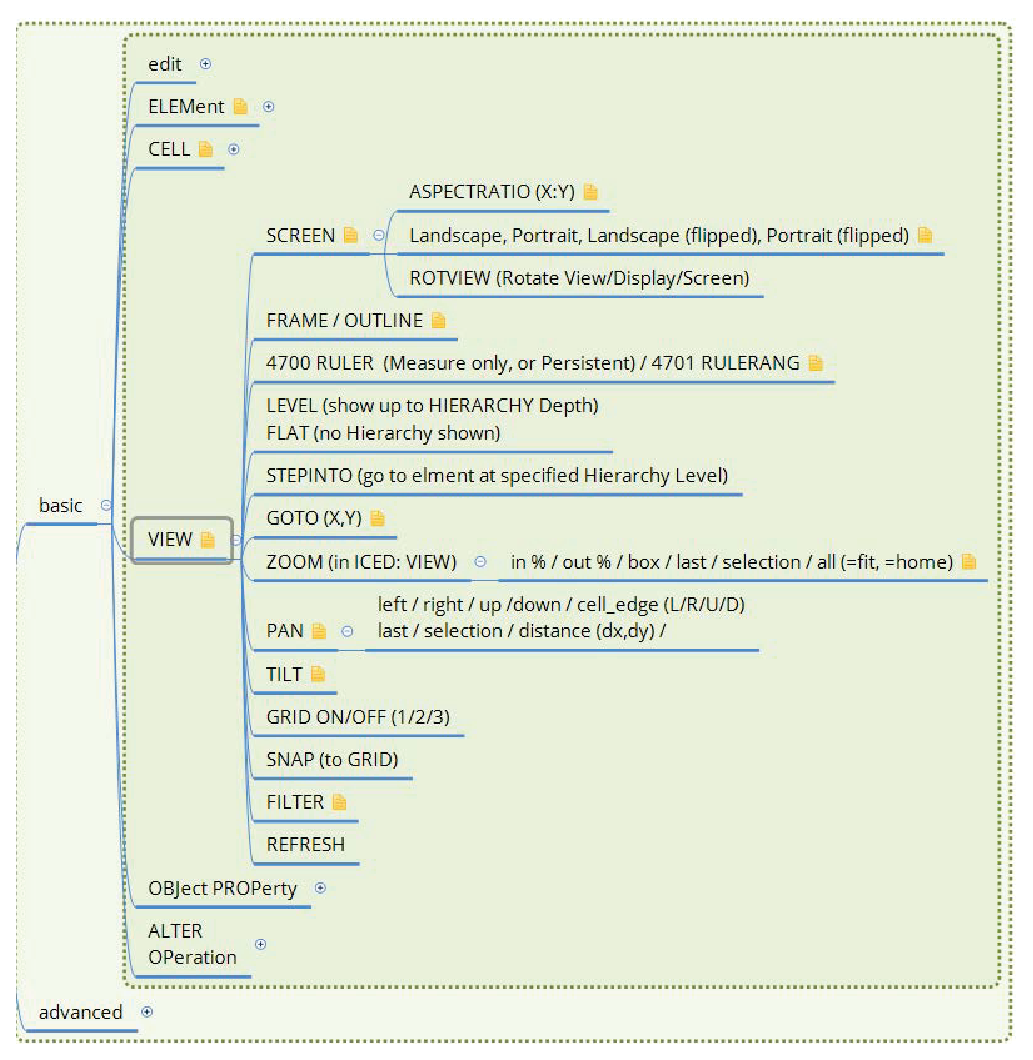
\includegraphics[width=4in]{./Layout/FigsCmd/CmdBasicView.eps}
	\caption{Commands to View Basic Elements 视图基本命令。}
	\label{FigCmdView}
\end{figure}
\subsubsection{屏幕设置(Screen)} \label{SectCmdViewScreen}
屏幕设置(Screen)调整屏幕的基本设置,比如纵宽比、页面设置、旋转设置。
\begin{itemize}
	\item Screen XtoY X Y  (设置屏幕纵宽比为X:Y)
	\item Screen Landscape (设置屏幕为横向)
	\item Screen Portrait  (设置屏幕为纵向)
	\item Screen Landscape flipped (设置屏幕为横向,左右颠倒)
	\item Screen Portrait  flipped (设置屏幕为纵向,上下颠倒)
	\item Screen Rotate    (设置屏幕旋转设定角度)
\end{itemize}

\subsubsection{边框显示(Frame/Outline)} \label{SectCmdViewFrame}
边框显示(Frame/Outline):显示或关闭基本图形和构元的边框
\begin{itemize}
	\item Frame On/Off   (显示或关闭基本图形和构元的边框)
	\item Outline On/Off (显示或关闭基本图形和构元的边框)
\end{itemize}

\subsubsection{标尺(Ruler)} \label{SectCmdViewRuler}
标尺(Ruler):显示或关闭测量的标尺。

RULER normally measures distance, but OptiMASK extents the ruler to angle measurement with 3 points, i.e., for consecutive 3 points A->B->C, the RULERANG tells the angle B.

支持厘米,毫米,英尺,英寸等多种刻度标尺。L-Edit use RULER as an annotation (which we defined in 4C01 NOTE)

\begin{itemize}
	\item Ruler On/Off   (显示或关闭测量的距离标尺)
	\item RulerAngle On/Off  (显示或关闭测量的角度标尺)
\end{itemize}

\subsubsection{层级深度(Level)} \label{SectCmdViewLevel}
层级(Level):显示构元引用层级深度(Hierarchy Level Depth)。程序可以设定最多层级256级,一般够用了。
\begin{itemize}
	\item View Level 1 to 10   (显示构元引用层级从第1级至第10级)
	\item View Flat 等同于 View Level 0 to 0  (显示所有构元列表,不分层级)
	\item GoTo Level 5 等同于 StepInto Level 5  (进入(激活)当前构元的子构元第5级)
\end{itemize}

\subsubsection{转至(GoTo)} \label{SectCmdViewGoTo}
转至(GoTo):转至指定的位置(Position)、构层(Layer)、构元(Cell)或者层级(Level)。
\begin{itemize}
	\item GoTo X Y   (转至指定的坐标位置(X,Y),即将此点设置为显示中心)
	\item GoTo Layer LAYERID/LAYERNAME (转至当前构元的指定构层)
	\item GoTo Cell  CELLID/CELLNAME (转至指定的构层)
	\item GoTo Level 5 (转至当前构元第5子级)
\end{itemize}

\subsubsection{缩放(Zoom)} \label{SectCmdViewZoom}
TILT, PAN, ZOOM are basic camera operations.

PAN -- Move Camera X or Y;

ZOOM -- Camera focus zoom in or out;

TILT -- Tilt the camera 

缩放(Zoom):缩放当前窗口的指定显示范围。缩放大小就用小数或者分数(包括$a/b$形式)表示。此处不用百分比符号\%,因为\%已经缺省允许为注释符号。
\begin{itemize}
	\item Zoom 0.80  (新视图是原视图的80\%,$<1$表示缩小)
	\item Zoom 1.20  (新视图是原视图的120\%,$>1$表示放大)
	\item Zoom in 1.20  (放大120\%,即新视图是原视图的120\%)
	\item Zoom out 1.20 (缩小120\%,即原视图是新视图的120\%)
	\item Zoom Box X0 Y0 X1 Y1  (新视图为矩形框选中的区域)
	\item Zoom Last  (转至上次的显示区域)
	\item Zoom Selection  (显示区域刚好包括所有选中的图元和构元)
	\item Zoom All  (显示区域显示当前构元的所有元素)
\end{itemize}

\subsubsection{平移(Pan)} \label{SectCmdViewPan}
平移(Pan):平移当前窗口的显示范围。平移时不改变显示的缩放。

When using keyboard <left>, <right>, <up>, <down>, the view change is panning. We allow command operation of panning as below:
\begin{itemize}
	\item Pan left/right/up/down  (显示范围左右上下移动1/4(缺省))
	\item Pan left/right/up/down 1/N (显示范围左右上下移动1/N,N为大于1的正整数)
	\item Pan cell (L/R/U/D)  (显示范围转至当前构元的左右上下边界)
	\item Pan Last  (转至上次的平移位置)
	\item Pan Selection  (移动至选中区域)
	\item Pan dX dY (显示中心移动(dX,dY))
\end{itemize}

\subsubsection{倾斜(Tilt)} \label{SectCmdViewTilt}
倾斜(Tilt):主要是3D图形时考虑,对于二维版图操作简单功能可以暂时不考虑。高级功能可以将二维版图操作倾斜指定视角。
\begin{itemize}
	\item Tilt AngleX AngleY AngleZ  (倾斜指定的(X,Y,Z)角度)
\end{itemize}

\subsubsection{格点(Grid)} \label{SectCmdViewGrid}
格点(Grid):显示或关闭显示屏上的格点。格点可以分多级(通常3或4级)。用户可任意定义每级格点的尺寸(缺省1/2/3/4级为1/0.1/0.01/0.001 user unit,比如\um)。
\begin{itemize}
	\item Grid On/Off   (显示或关闭显示屏上的各级格点)
	\item Grid 1/2/3/4 On/Off (显示或关闭显示屏上的指定级别的格点)
	\item Grid 4 Size 0.001 (第四级格点设置为0.001 user unit;其它级别类似设置)
\end{itemize}

\subsubsection{对格(Snap)} \label{SectCmdViewSnap}
对格(Snap): see \emph{ICED™ Command File Programmer's Reference}
\begin{verbatim} C:\icwin\doc\LAYOUT_PROGRAMMER_REF.PDF \end{verbatim} 

There are snap grid and snap angle parameters that control how you can digitize points with the cursor。

Coordinates in an ADD command will NOT be forced to lie on the resolution or
snap grids. When coordinates are digitized using the mouse, then you can be
sure that the coordinates are on the snap and resolution grids. However, if your
command file uses mathematical operations to calculate coordinates, they
probably do not lie on grid. You will need to perform extra processing to snap
the coordinates to grid before using them in an ADD command.

If you calculate coordinates, you should use the functions below to snap the
coordinates to grid. If you prefer to avoid rounding coordinates to grid, your
command file should check the value of the system macro RES.MODE to
determine if the user has set the resolution mode to "SOFT". If the resolution mode is "SOFT", then the decision is up to you.

However, if the resolution mode is "HARD" then the user has indicated that all
coordinates should be on grid.

The ROUND() function is usually used to round a coordinate pair to the nearest
point on the resolution grid. 

\subsubsection{过滤(Filter)} \label{SectCmdViewFltr}
过滤(Filter):只显示符合条件的图元或者构元。Advanced capability, not need in minimum version. Only show objects that satisfy the filter criteria. 
\begin{itemize}
	\item View Filter Show CellName Contain CHAR (仅显示构元名字包含指定字符的构元)
\end{itemize}

\subsubsection{刷新(Refresh)} \label{SectCmdViewRefresh}
刷新(Refresh):刷新当前视图。有时可能操作后,没有及时刷新显示,那么就强制用刷新(Refresh)命令重现显示。 
\begin{itemize}
	\item View Refresh (刷新当前视图显示)
\end{itemize}

\subsection{属性(Object Property))} \label{SectCmdProperty}

\subsection{变化(Alter)} \label{SectCmdCell}

\subsection{注意} \label{SectCmdNote} 
命令和脚本注意事项。

%%\pagestyle{empty}
%%\cleardoublepage
%%to generates one blank page for the next chapter to be on an odd page
